\section{Introduction}
\paragraph{History}
\begin{itemize}
	\item First, thermodynamics was developed, before atoms were known to exist.
	\item Statistical physics.
	\item Quantum physics. 
\end{itemize}
In the course, the order is the opposite.
\subsection{}
Suppose we have two balls of diameter $d$. If both are on the bottom, total energy is 0. If one i son the other, total energy is $mgd$.

\begin{center}
	\includegraphics[width=0.5\linewidth]{./lect1/pic1.png}
	
	\begin{tabular}{c|c|c}
		Number of state & Degeneracy & Energy \\\hline
		0 & 3 & 0 \\
		1 & 3 & $mgd$ \\
		2 & 0 & $2mgd$ \\
	\end{tabular}
\end{center}
\paragraph{Paramagnetism}
Define magnetic moment as $\vec{m} = I \vec{a}$.
For magnetic filed energy is $U = -\vec{B} \cdot \vec{m} = - \vec{B} \dot \vec{\mu}$.

Suppose we a have a system of a big amount of current loops, each of which can have one of two directions - clockwise or counterclockwise. For example

\begin{center}
	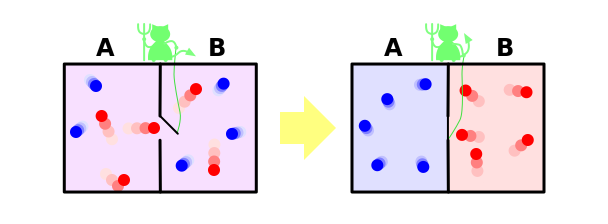
\includegraphics[width=0.5\linewidth]{./lect1/pic2.png}
\end{center}
To calculate total magnetic momentum we just sum all of the moments, which are either $\mu$ or $-\mu$. In upper example, $M = \sum_i \mu_i = 2\mu$.


The total number of possible states is $2^N$. The possible energy is $M = (N-2N_d)\mu$ where $N_d$ is number of down-facing loops of current. Number of different states with sam energy is $$\binom{N}{N_d} = \frac{N!}{N_d!N_u!}$$

Now, for even $N$, define 
$$2S = N_u -N_d$$
Then
$$\binom{N}{N_d} = \frac{N!}{(\left(\frac{1}{2} N - S\right)!(\left(\frac{1}{2} N + S\right)!}$$
and the energy
$$U = -2S\mu B \Rightarrow S = -\frac{U}{2\mu B}$$
The degeneracy of the state thus is
$$g(N,S) = \frac{N!}{\left(\frac{1}{2} N - \frac{U}{2\mu B}\right)!(\left(\frac{1}{2} N + \frac{U}{2\mu B}\right)!}$$ 
\paragraph{Particles on shelves (quantum oscillator)}
Suppose we have equally-distant shelves, and energy distance between two shelves is $\epsilon_0$:
\begin{center}
	\includegraphics[width=0.5\linewidth]{./lect1/pic3.png}
\end{center}
Define $n=\frac{U}{\epsilon_0}$ which is amount of energy we have (it comes in quantas is degeneracy? What is degeneracy? It is combinations of$N$ out $n$ with returns:
$$g(N,u) = \frac{(n+N-1)!}{n!(N-1)!} = \frac{\left(N+\frac{U}{\epsilon_0} - 1\right)!}{\left(\frac{U}{\epsilon_0}\right)!(N-1)!}$$

\paragraph{Particles on shelves with quadratic distances (particles in box)}
Now suppose distances goes as square of number opf shelve ($\epsilon_0$, $4\epsilon_0$, ...). This problem doesn't have analytical solution. But we can find solution manually. For example, to find $g(6,18\epsilon_0)$. The only option is 2 boxes on first energy level $U=\epsilon_0$ and 4 on second energy level, thus 
$$g(6, 18\epsilon_0) = \binom{6}{2}=15$$  
\paragraph{1D box with particles}
Now we want to calculate kinetic energy:
$$E = \frac{p^2}{2m}$$
Since we can't do much with continuous values (there is infinite number of options), lets divide both momentum and position into discrete intervals of size $w$ and $l$ correspondingly. Now, the position is independent on energy, but there are only two options for momentum - $\pm \sqrt{2mE}$. Thus degeneracy is
$$g(1, E) = 2\frac{L}{l} $$
\paragraph{2D box}
We now divide position in momentum into intervals of length $l$ and $w$ in both directions. Position is still arbitrary, and momentum lies on a circle of radius $2mE$. However, its hard to calculate.

Lets define instead $S(1,E)$ - number of states with energy \textit{less} than $U$. For 1-dimensional case 
$$S(1,E)  = \frac{L}{l} \cdot 2 \cdot \frac{\sqrt{2mE}}{w} = \frac{1}{lw} \int_{-\frac{L}{2}}^{\frac{L}{2}} ds \int_{-\sqrt{2mE}}^{\sqrt{2mE}} ds$$
In 2D we get, for box of area $A$
$$S(1,E) = \frac{A}{l^2} \cdot \frac{2\pi m E}{w^2} =  \frac{1}{l^2w^2} \int_{-\frac{L}{2}}^{\frac{L}{2}}dx\int_{-\frac{L}{2}}^{\frac{L}{2}}dy \iint\limits_{|p| < \sqrt{2mE}} d^2p$$
$$S(1,E) = \frac{V}{l^3} \cdot\frac{4\pi (2 m E)^{\frac{3}{2}}}{3w^3}$$
We denote $h=lw$.